% ************************************************************************
%
% Introduction
%
% ************************************************************************
\hyphenation{theory} %% in one place the word theory was wrongly
                     %% hyphenated , the-ory

\myquote{0.7\textwidth}{Anyone who does not look back to the beginning
  throughout a course of action, does not look forward to the end.
  Hence it necessarily follows that an intention which looks ahead,
  depends on a recollection which looks back.}{Aurelius Augustinus,
  \emph{De civitate Dei}, VII.7 (\oldstylenums{417}
  A.D.)\nocite{Augustin-DeCivitateDei}}

\noquote


\chpos{22mm}{10mm}
\chapter[Introduction]{Introduction}
\markboth{\thechapter\ \ Introduction}{\thechapter\ \ Introduction}
\label{chapter1}

\mysquote{\textwidth}
{There are two possible outcomes: If the result confirms the hypothesis, then you've made a measurement. If the result is contrary to the hypothesis, then you've made a discovery.}
{Enrico Fermi (1901--1954)}


% ************************************************************************
\section{Studying Neuron Cell} 
Some text \cite{abramoff2004image}. And \cite{ascolitrees}.


\section{Thesis Outline}

%\begin{figure}[!t]
%  \begin{center}
%  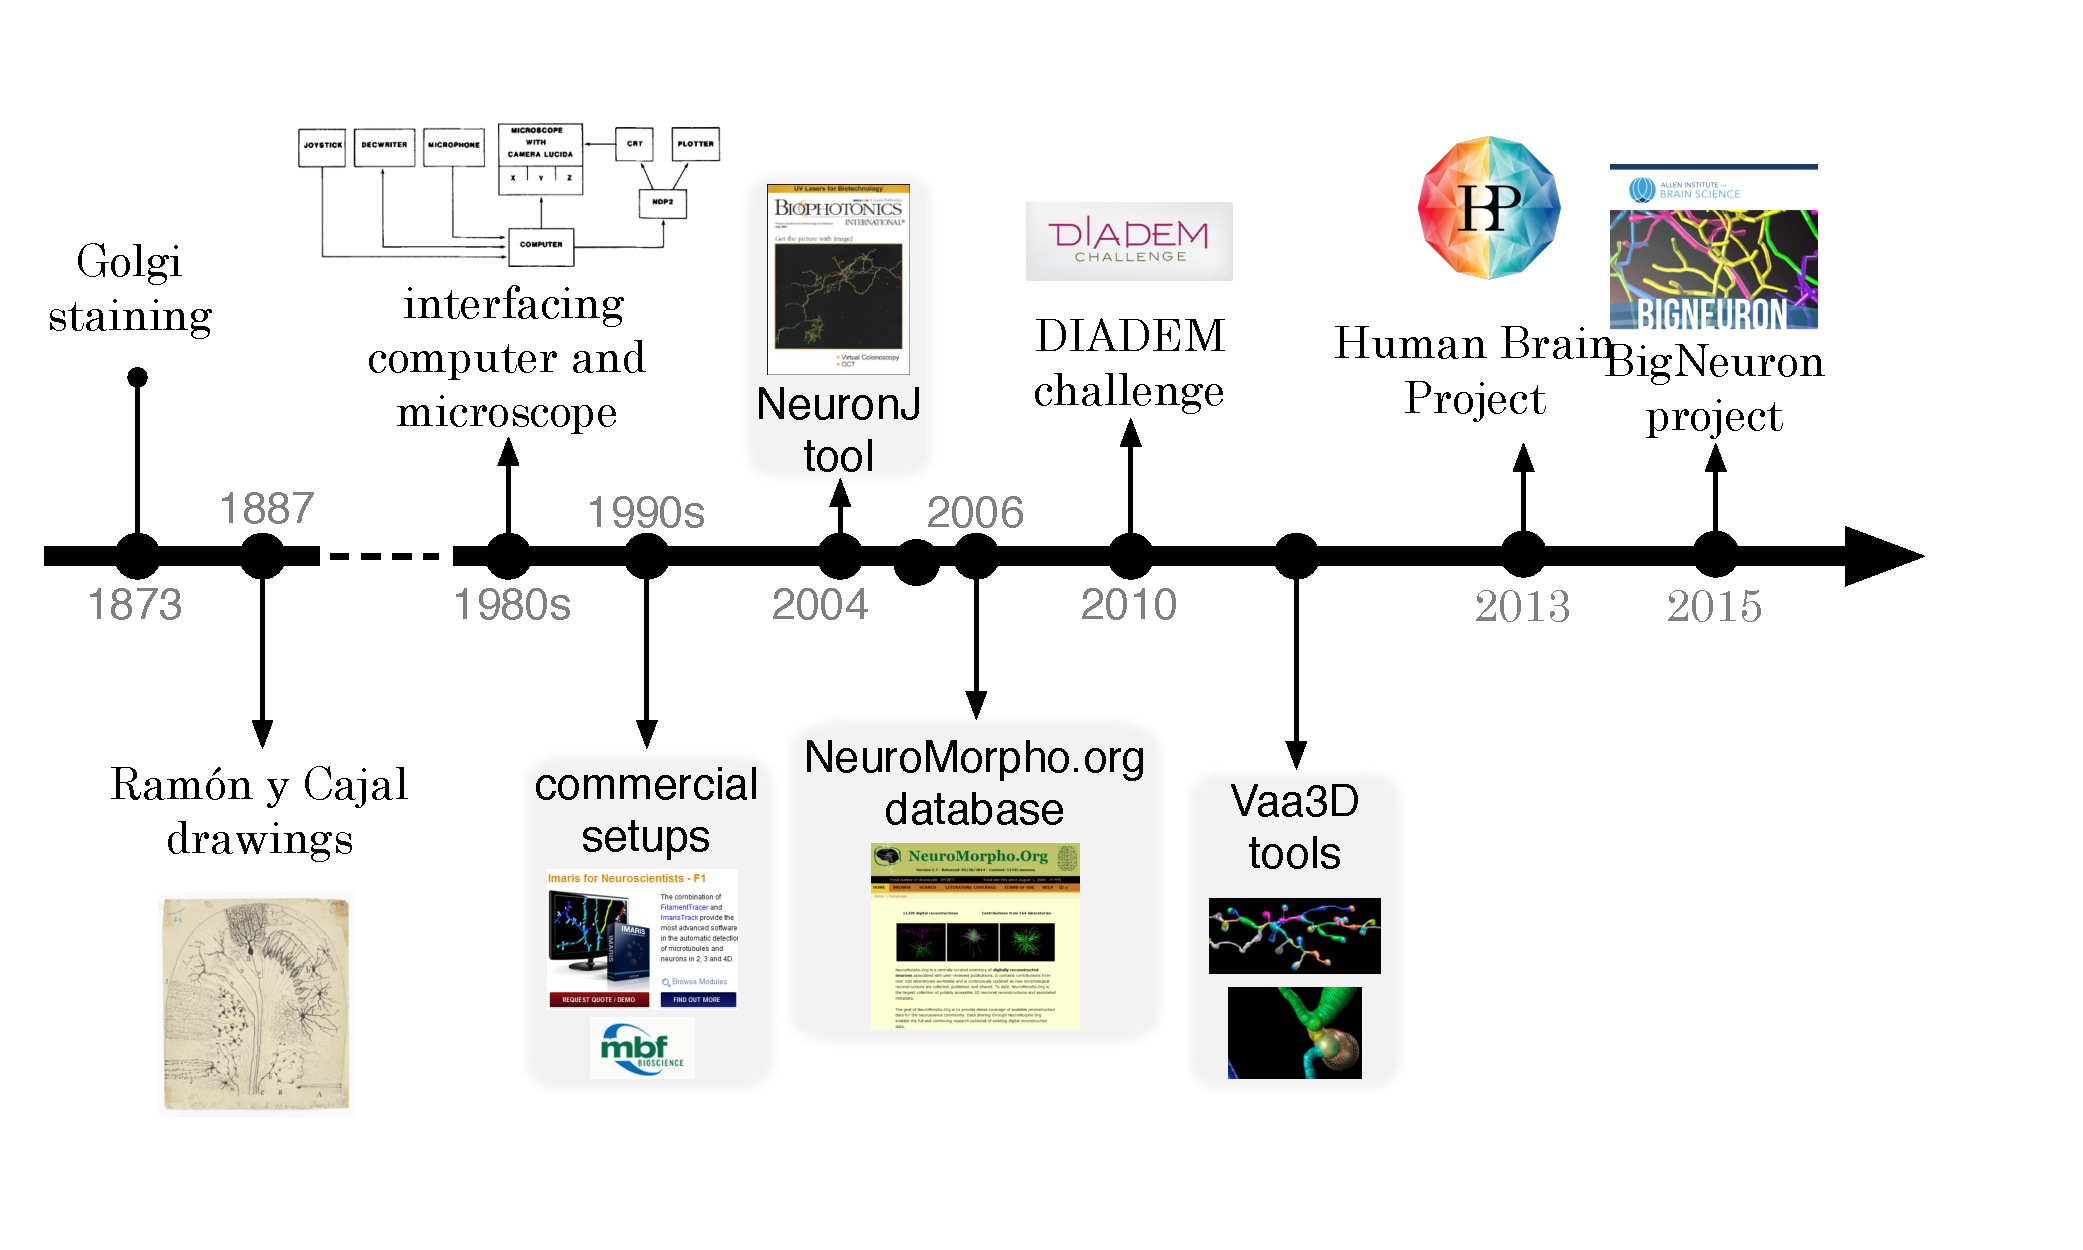
\includegraphics[width=\textwidth]{ch1_fig1}
%  \end{center}
%\vspace{-3ex}
%  \caption{Examples of images acquired for different biological
%    studies based on GFP labeling and fluorescence
%    microscopy. The images are single frames from 2D time-lapse
%    studies of activity of microtubule plus-ends (top left), microtubule
%    plus-ends in neurons (top right), Rab5 (bottom left) and
%    peroxisomes (bottom right).
%}
%\vspace{-1ex}
%\label{ch1__fig1}
%\end{figure}
